\documentclass[12pt,a4paper]{article}
\usepackage{latexsym}
\usepackage{amsmath}
\usepackage[dvips]{graphicx}
\usepackage{times}
 \usepackage[center]{subfigure}
  \usepackage[Algorithme]{algorithm}		% 		\begin{algorithm}
  \usepackage{algorithmic}						% 		\begin{algorithmic}
\usepackage{placeins}
\usepackage{mdwlist}								% for a compact itemize

\RequirePackage[singlelinecheck=off]{caption}
\captionsetup{singlelinecheck=on}
\captionsetup{justification=centering}

\textwidth =  144mm
\textheight = 226mm
\headheight 4mm
\headsep = 7mm
\footskip = 13mm
\parindent  = 5mm
\parskip = 1 mm
\oddsidemargin = 7.6mm
\evensidemargin = 7.6mm
\topmargin -.4mm
\pagestyle{plain}
\pagenumbering{arabic}

\title{Article - PGD approach for low frequency dynamics problems}
\author{Pierre \bsc{Nargil}}
\date{8^{th} april 2013}

\flushbottom

\begin{document}
\noindent \vspace*{70.0mm}
\subsection*{Abstract}
Answering the need of an industrial looking for a model order reduction to use on a parametric problem, we offer to adapt the proper generalized decomposition (PGD) for its use. The goal of this work is to adapt the PGD to dynamics problems. The proper orthogonal decomposition (POD) will be used as a comparison tool for the PGD basis, as they are both reduced order modeling methods using separated variables. In order to use these methods on dynamics problems, a choice has to be made regarding the integration scheme, therefore this paper will present different possibilities and show what they offer. Results on academical problems of the method will be presented.
 
\vspace{0.2in}
\noindent{\bf Keywords:} Reduced Order Modeling, Separated variables representation, PGD, POD, dynamics, Reduced Basis.


\section{Introduction}


This work originated from an industrial need, regarding a time consuming simulation. The industrial runs a complex numerical model simulating the behavior of a car on the road. This non-linear slow dynamics problem takes a time to be solved measured in days, and it has to be ran numerous times to evaluate the car response for different sets of parameters. This is why a reduced order modeling method is needed. The PGD has been chosen since it allows to introduce parameters inside the problem, and provides a solution for all values of the parameters.

This work takes place among the model order reduction methods. The PGD method is the center of many current studies, applying its use to various cases. This paper will be centered on dynamics problems.

The need to be competitive brings more and more industrials to head towards simulation tools, which allow, at least during conception, to reduce the prototypes try-outs and therefore to decrease the time and cost of development.

It also enabled technical research offices to use optimization on conception and to produce probabilistic models. These two processes have in common their high cost in resources and calculation time, since both need the assessment of numerous solutions of the numerical model. That is why they are currently applied only to quite simple models in the industrial world. To deal with large problems, it is necessary to reduce calculation time while preserving a reasonable quality through model order reduction strategies.

Among the various methods of model order reduction existing, we offer to work essentially on the PGD \cite{ladeveze1999nonlinear,Multidimensional,ShortReview}. Originally developed to solve evolution problems within the LATIN \cite{ladeveze1989latin}, this method has known numerous evolutions the past few years \cite{ElasticVisco,Parametrized}: Multiscale in space and time, stochastic use, parametric problems, "optimal" PGD base construction... This family of model order reduction using a representation with separation of variables is said \textit{a priori}, since the reduced basis are built on the fly without the need for the exact solution of the problem (not even an approximation of it). The principle is to find the decomposition of the solution of a problem as a sum of products of separated variables functions (variables can represent a parameter of the problem \cite{Multidimensional}). In our case, the problem depends on the values of a set of parameters, and using the PGD ability to add parameters as variables, the resolution will provide a solution for all values of each parameter introduced this way.

In this paper, our goal is to apply this method to dynamics problem presenting non-linearities. We will provide a comparison with another model order reduction method, the POD \cite{Chatterjee}. This method will allow us to compare solutions but also reduced basis. The POD can be attached to the singular value decomposition (SVD) and as such it guarantees a form of optimality of the reduced basis, but this method has the major drawback to be \textit{a posteriori}, implying that the method is applied to a previous resolution of the complete system. This means that a first resolution is required on the complete basis and that the acquired reduced basis is linked to this resolution.

An application of the PGD in the case of linear dynamics problems on academic examples will be presented comparing it to POD results. It will illustrate the performances and advantages of this method, showing the influence of the loading velocity, emphasising the results of integration scheme choice such as Galerkin time discontinuous \cite{GDDisc} and pointing out the importance of orthogonalization.



\subsection{POD}
\label{IntroPOD}
The proper orthogonal decomposition (POD \cite{Chatterjee}), known previously as principal component analysis (PCA \cite{PCA}) or Karhunen-Loeve (K-L \cite{kittler1973new}) expansion, enables to extract from great quantities of data, the principal modes: the best representing the whole set of data. It is linked to the SVD, which could be seen as its discrete version. The SVD has for example been used in former face recognition programs.

\subsubsection{Singular Value Decomposition}

$\mathbf{A} (n \times m)$ being a matrix, there are $\mathbf{U} (n \times n)$, $\mathbf{V} (m \times m)$ orthogonal and $\mathbf{S} (n \times m)$ diagonal with coefficients zeros or positive numbers, such as:
\begin{equation}
\mathbf{A} = \mathbf{U}\mathbf{S}\mathbf{V}^T
~~~A_{ij} = \mathbf{u_i} \mathbf{S} \mathbf{v_j}^T
~~~\text{where }\mathbf{u_i}\text{ et }\mathbf{v_j}\text{ are the lines of }\mathbf{U}\text{ and }\mathbf{V}
\end{equation}

This decomposition is not unique, but for $\mathbf{S}$ to be, it is chosen as a convention to order the values on its diagonal decreasingly: $S_{ii} \geq S_{(i+1)(i+1)}$. These values are called singular values and for a matrix $\mathbf{A}$ having for rank $r$: 
$S_{ii} = 0~ \forall i > r$. The decomposition can then be truncated at the order $r$ (see below). Note: $r$ $\leq$ $min(m, n)$.

These singular values are not without reminding the eigenvalues, and they are linked to them. It can be noted that singular values can be calculated for rectangular matrices but eigenvalues only exist for endomorphisms so they are limited to square matrices. The relation between the two decompositions is that $\mathbf{V}$ contains the eigenvectors of $\mathbf{A}^T \mathbf{A}$ (symmetrically $\mathbf{U}$ contains the eigenvectors of $\mathbf{A}\mathbf{A}^T$). And the squares of singular values of $\mathbf{A}$ are the modulus of the eigenvalues of $\mathbf{A}\mathbf{A}^T$. If $\mathbf{A}$ is symmetrical positive, its eigenvalues are its singular values and $\mathbf{U}$ = $\mathbf{V}$. If $\mathbf{A}$ is symmetrical but has some negative eigenvalues, then its singular values associated to these columns will be their absolute values.
\subsubsection{Truncated SVD}
The goal of this decomposition is to reduce the quantity of data keeping as good as possible the information it was containing. The left and right singular vectors (respectively the columns of $\mathbf{U}$ and $\mathbf{V}$) give modes as representative of the whole set of data as they are associated with higher singular values. An order $k$ is chosen to keep only the highest singular values.
\begin{equation}
\begin{array}{c}
\mathbf{A}^{(k)} = \mathbf{U} \mathbf{S^{(k)}} \mathbf{V}^T
~~~A_{ij} = \mathbf{u_i} \mathbf{S^{(k)}} \mathbf{v_j}^T
\\
\text{where } \text{S}^{(k)}_{ij} = \text{S}_{ij} ~~ \forall i,j < k \text{, and zero above}
\end{array}
\end{equation}
this gives the approximated matrix $\mathbf{A^{(k)}}$, but then a big part of the system $\mathbf{U} \mathbf{S^{(k)}} \mathbf{V}^T$ is useless since it brings no contribution to the result because of multiplication with zeros of $\mathbf{S^{(k)}}$. Therefore each matrix can be truncated. Here is to visualize the $k$ order truncation effect:
\begin{equation}
\begin{matrix}
	&
	\begin{bmatrix}
	   S_{11} &\cdots& 0 \\
	   \vdots &\ddots& \vdots \\
	   0 &\cdots& S_{kk} \\
	\end{bmatrix}
	&
	\begin{bmatrix}
	   V_{11} &\cdots& V_{m1} \\
	   \vdots &\ddots& \vdots \\
	   V_{1k} &\cdots& V_{mk} \\
	\end{bmatrix}
\\
	\begin{bmatrix}
	   U_{11} &\cdots& U_{1k} \\
	   \vdots &\ddots& \vdots \\
	   U_{n1} &\cdots& U_{nk} \\
	\end{bmatrix}
	&
	(n \times k) 
	&
	(n \times m)
\end{matrix}
\end{equation}

$\mathbf{U}$ and $\mathbf{V}$ are truncated after their $k^{th}$ column, and $\mathbf{S}$ after its $k^{th}$ line and its  $k^{th}$ column, but $\mathbf{A^{(k)}}$ stays the same size as $\mathbf{A}$.

Obviously the quicker the singular values decrease the more efficient the truncation will be.

The SVD assures the optimality of the approximation, because the matrix obtained after truncation of order $k$, is the matrix of rank $k$ which minimizes the error: $  \Vert \mathbf{A} - \mathbf{A}^{(k)} \Vert_F$. The Frobenius norm is equal to the square root of the sum of all the squared terms of a matrix, which is also equal to the highest singular value.

The truncated SVD still needs the computation of the full SVD, which represents a number of numerical operations the same order as $O(mn^2)$, directly linked to the calculation time. And even if it is transposed to exchange the role of $m$ and $n$, it represents a handicap which amplifies at the same time as the size of the studied matrix. To fight this issue, approximated decomposition methods have been developed, the low-rank matrix approximation method (LRMA), and particularly the QUIC-SVD, which allows to control the error caused by the approximation \cite{QUIC-SVD}.

The POD is generally used in its discrete version, because data basis are discrete (like for example due to experimental sampling), or simply because of the discretization used by numerical solvers. A use of the continuous form can be found in \cite{Turbulence}, it will be described in the next part.

\subsubsection{Continuous formulation}
The POD is a method which offers a solution with separated variables in the form of a sum of product of functions. $z(x,t)$ will be approximated in this form:
\begin{equation}
\label{DecompoPOD}
z(x,t) \approx \sum_{k=1}^m a_k(t) \varphi_k(x)
\end{equation}

In the rest of this paper, $x$ will represent the space coordinate (so it can be a vector) and $t$ the time coordinate. The decomposition \ref{DecompoPOD} is not unique since the space containing the functions $\varphi_k(x)$ has to be chosen. For example if $x$ is inside an interval of real numbers $\Omega$,  then the functions $\varphi_k(x)$ can be chosen as Fourier series, Legendre polynomials, Tchebychev polynomials, etc... And this choice influences obviously the result obtained for the functions $a_k(t)$. The hypothesis is made that the space approximation for the space functions is well chosen and that the sum will approach the solution $z(x,t)$ when $m$ approaches infinity (more precisely on the definition domain of $z(x,t)$, apart from potential ensembles of measure zero, reader which are not familiar with measurement theories can read \cite{Analysis}. This consideration will not be developed here. The same goes for the questions of integrability of the functions, which is no problem in discrete calculation)

If for $\varphi_k(x)$ functions an orthonormal basis is chosen, we have:
\begin{equation}
\int_\Omega \varphi_i(x) \varphi_j(x) dx = \delta_{ij}
\end{equation}

\noindent
We obtain the following formula for $a_k(t)$:
\begin{equation}
	a_k(t) = \int_\Omega z(x,t) \varphi_k(x) dx 
\end{equation}
then the determination of the function $a_k(t)$ only depends on $\varphi_k(x)$.

If the decomposition is optimal, i.e. if for each term of the sum there is no better approximation, then the terms are called proper orthogonal nodes, and the sum proper orthogonal decomposition.

\noindent
To match with the discrete formulation, we define:
\begin{equation}
	\mathbf{A} 	= \mathbf{Q} \mathbf{V}^T 
				= \sum_{i=1}^m \mathbf{q_i} \mathbf{v_i}^T
		\text{ where } \mathbf{Q} = \mathbf{U}\mathbf{S}
\end{equation}

In this discrete form of the equation \ref{DecompoPOD}, the matrix $\mathbf{A}$ represents $z(x,t)$ and the columns $\mathbf{q_i}$ represent the functions $a_k(t)$. 
The link between singular values and eigenvalues has been described previously, and this connection can help solving this problem. We define $\mathbf{B} = \mathbf{A}^T \mathbf{A}$, which will give in the case of continuous time but discrete space representation:
\begin{equation}
	\text{B}_{ij} = \frac{1}{T} 
			\int_{t_0}^{t_0+T} z(x_i,t) z(x_j,t)dz
\end{equation}

And if we change to infinite dimension formulation, there are an infinity of eigenvalues and B is no longer a matrix but a function of two variables:
\begin{equation}
	B(x_1,x_2) = \frac{1}{T} 
			\int_{t_0}^{t_0+T} z(x_1,t) z(x_2,t)dz
\end{equation}
where $x_1$ and $x_2$ are continuous variables defined on $\Omega$. 

$\boldsymbol{\psi}$ being an eigenvector of $\mathbf{B}$, of eigenvalue associated $\lambda$, then $\mathbf{B}\boldsymbol{\psi} = \lambda\boldsymbol{\psi}$. Which gives in discrete form:
\begin{equation}
\sum^m_{j=1} \text{B}_{ij} \psi_j^T = \lambda\psi_i
\end{equation}
and becomes an integral in continuous form:
\begin{equation}
\int_\Omega B(x_1,x_2) \psi(x_2) dx_2 = \lambda\psi(x_1 )
\end{equation}

One of the problem of this model order reduction method \textit{a posteriori} is that it depends on the solution obtain previously. Indeed the modes found are representing the original data, and if in the calculation, the configuration of the considered system should change, the modes would not be correctly representing the solution. The separated variables representation used by the POD also has limits, in particular the bad representation of a local perturbation that moves, typically a wave propagating (the solution of the d'Alembert equation is not with separated variables $f(x \pm \beta t )$).


\subsection{PGD}
Like the POD, the proper generalized decomposition (PGD \cite{Multidimensional}) approximate the solution, using the hypothesis of separated variables, as a sum of products of functions. A function $ z(x,t)$ would be represented in the following form:
\begin{equation}
z(x,t) \approx \sum^m_{k=1} a_k(t) \varphi_k(x)
\end{equation}

It was originally introduce by \cite{ladeveze1999nonlinear} within the LATIN method. It differs from the POD since the function $ z(x,t)$ is unknown at the start. The modes are not known previously to the resolution, they are calculated "on the fly" thanks to an algorithm as such :
%"algorithme des puissances itérées"

\begin{center}
\begin{algorithm}
\caption{PGD Resolution}
\begin{algorithmic}[1]
\FOR{$m = 1 $ to $ m_{max}$}
\STATE initialize $a_1$
\FOR{$k = 1 $ to $ k_{max}$}
\STATE $\varphi_k \leftarrow S_m(a_k )$
\STATE norm $\varphi_k$ ($\Vert\varphi_k\Vert_\Omega = 1$)
\STATE $a_k \leftarrow T_m (\varphi_k )$
\STATE check the convergence of $(\varphi_k a_k)$
\ENDFOR
\STATE $\varphi_m \leftarrow \varphi_k$ and $a_m \leftarrow a_k$
\STATE $z_m = z_{m-1} + \varphi_m a_m$
\ENDFOR
\end{algorithmic}
\label{AlgoPGD}
\end{algorithm}
\label{AlgoPGDPartie}
\end{center}


Where $\text{S}_m$ is the application associating to a time function $a$, a space function $\varphi$. And $\text{T}_m$ the application associating to a space function $\varphi$, a time function $a$. To find them we start with the weak formulation of the problem:
\begin{equation}
\label{ProblemeLM}
B(u,v) = L(v) ~~ \forall v \in H
\end{equation}

Where $H$ is a Hilbert space, $B$ a bilinear form, continuous and coercive on $H$ and $L$ a linear form continuous on $H$.

A classical process is applied for the PGD, called Galerkin progressive: $z_{m-1}$ (the approximation of $z$ at the order $m-1$) is supposed known. The goal is to find a new couple $(\varphi, a) \in  U \times V$. It is defined as the one verifying the criterion of double orthogonality of Galerkin, i.e.:
\begin{equation}
\label{formulationFaible}
B(z_{m-1} + \varphi a , \varphi a^* + \varphi^*  a) = L (\varphi a^* + \varphi^* a) ~~~
\forall \varphi^*  \in U \text{ et } \forall a^* \in V 
\end{equation}
Then $S_m (a)$ is defined by:
\begin{equation}
B(z_{m-1} + \varphi a , \varphi^*  a) = L (\varphi^* a) ~~~
\forall \varphi^*  \in U
\end{equation}
and $T_m (\varphi)$ by:
\begin{equation}
B(z_{m-1} + \varphi a , \varphi a^*) = L (\varphi a^* ) ~~~
\forall a^* \in V 
\end{equation}

The couple  $(\varphi, a)$ verifies the equation \ref{formulationFaible} if and only if $\varphi = S_m (a)$ and $a = T_m (\varphi)$, which is a non-linear problem, of which the resolution by the PGD can be seen as an eigenvalues problem where $\varphi$ and $a$ are respectively the dominant eigenfunctions of $S_m \circ T_m$ and $T_m \circ S_m$. Allowing to draw our inspiration from algorithms used in eigenvalues problems and giving the algorithm 1, which provides the decomposition.  It can be modified, in particular to add the orthogonalization which can improve the quality of the basis found (it works as long as there are only two variables). If we want to orthogonalize $\varphi_m$ with the existing basis \{$\varphi_1 , \varphi_2 , ... , \varphi_{m-1}$\}, a dot product needs to be defined, for example such as:

\begin{equation}
\langle u,v \rangle_\Omega = \int_\Omega \! uv ~ d\Omega
\end{equation}


\section{Dynamics}
\noindent
The fundamental equation of dynamics is verified at any time:
\[
\mathbf{M}\mathbf{\ddot{u}} + \mathbf{C}\mathbf{\dot{u}} + \mathbf{K}\mathbf{u} =
\mathbf{f}
\]

It is a differential equation in $\mathbf{u}$. In order to solve a differential equation there are different methods. Ideally there is one that gives an exact and explicit solution, but it is limited to a few classical cases. But in general cases differential equations are solved approximately and numerically. It relies on the discretization of the response domain. In space it means creating a mesh, allowing to define quantities depending on space as matrices. Time representing only one dimension, a simple choice of a fixed time step to slice the time domain, enables to represent it more or less precisely.

\subsection{Integration scheme}
\label{SchemasDIntegration}

The discretization of the time axis allows to solve the equation at a given instant (provided that the solution is known at the previous instant*). In order to do so, a choice of a differentiation method has to made to derive $\mathbf{u}$, therefore a numerical scheme is chosen.

\noindent *If a scheme only uses the solution at the previous time step and not the ones before it, it is said to use a unique step, otherwise it is said to use multiples steps.

In order to describe the differentiation of a discrete function, we can use the Euler scheme, Runge-Kutta's or Crank-Nicholson's. In the particular case of dynamics the Newmark method is used to define the links between acceleration, velocity and displacement. These links are defined by two equations using parameters which can make the algorithm explicit or implicit, and influence its stability.

A scheme is said to be stable if it can control the accumulation of calculation error. Some schemes are conditionally stable and the solution they provide can diverge. The condition of stability in dynamics is generally a condition on the discretization of time: choosing a time step that is not too small to define the propagation of information in the mesh elements. The critical size above which the time step must not be, is therefore depending on the size of the mesh elements.

\subsubsection{Newmark method}

The method introduced by \cite{Newmark} gives an integration scheme based on two equations:
\begin{equation}
\label{Newmark1}
	\mathbf{u_{n+1}} = \mathbf{u_n} + dt.\mathbf{\dot{u}_n}
	+ \frac{dt^2}{2}[(1-2\beta)\mathbf{\ddot{u}_n} + 2\beta\mathbf{\ddot{u}_{n+1}}]
\end{equation}
\begin{equation}
\label{Newmark2}
	\mathbf{\dot{u}_{n+1}} = \mathbf{\dot{u}_n} 
	+ dt[(1-\gamma)\mathbf{\ddot{u}_n} + \gamma \mathbf{\ddot{u}_{n+1}}]
\end{equation}

\noindent
The scheme stability depends on the two parameters $\beta$ and $\gamma$:
\begin{center}
\begin{tabular}{c c}
$\gamma \leq 1/2$
& Unstable\\
$\gamma \geq 1/2 \text{ et } 2 \beta \leq \gamma$
& Conditionally stable\\
$\gamma \geq 1/2 \text{ et } 2 \beta \geq \gamma$
& Unconditionally stable\\
\end{tabular}
\end{center}

\noindent
For particular sets of values we find the usual methods:
\begin{center}
\begin{tabular}{c c c c}
\textbf{Name} & $\boldsymbol{\gamma}$ & $\boldsymbol{\beta}$ & \textbf{Properties}\\
\hline
Centered Differences&1/2&0&Explicit and Conditionally stable\\
Fox Goodwin&1/2&1/12&Conditionally stable\\
Linear Acceleration&1/2&1/6&Conditionally stable\\
Average Acceleration&1/2&1/4&Unconditionally stable\\
\end{tabular}
\end{center}

\noindent
The equation of dynamics can be written this way:
\begin{equation}
	\mathbf{M} \mathbf{\ddot{u}} + \mathbf{C} \mathbf{\dot{u}} + \mathbf{K} \mathbf{u} = \mathbf{f}
\end{equation}

\noindent
Which gives, when associated with equations \ref{Newmark1} and \ref{Newmark2}, if $\mathbf{K}$ does not depend on $\mathbf{u}$:
\begingroup\small
\begin{equation}
	\begin{array}{c}
	\overbrace{(\mathbf{M}+\mathbf{C} \gamma dt + \mathbf{K}\beta dt^2)}^{\mathbf{S}} \mathbf{\ddot{u}_{n+1}} 
	= 
	\\
	\mathbf{f_{n+1}} 
	- \mathbf{C}\overbrace	{
						[\mathbf{\dot{u}_n} + dt (1-\gamma) \mathbf{\ddot{u}_n}]
					}
					^{\mathbf{\dot{u}^p_{n+1}}}
	-\mathbf{K}\overbrace	{
						[\mathbf{u_n} + dt \mathbf{\dot{u}_n} 
						 + \frac{dt^2}{2} (1-2\beta) \mathbf{\ddot{u}_n}]
					}
					^{\mathbf{u^p_{n+1}}}
	\end{array}
\end{equation}
\endgroup

\noindent
Allowing to find in three steps, the values of $\mathbf{\ddot{u}}$, $\mathbf{\dot{u}}$ and $\mathbf{u}$:
\begin{equation}
	\left\{
		\begin{array}{r c l}
			\mathbf{\ddot{u}_{n+1}} 
			&=& \mathbf{S}^{-1} (  \mathbf{f_{n+1}} - \mathbf{C} \mathbf{\dot{u}^p_{n+1}} - \mathbf{K} \mathbf{u^p_{n+1}}  )
			\\
			\mathbf{\dot{u}_{n+1}} &=& \mathbf{\dot{u}^p_{n+1}} + dt \gamma \mathbf{\ddot{u}_{n+1}}
			\\
			\mathbf{u_{n+1}} &=& \mathbf{u^p_{n+1}} + dt^2 \beta \mathbf{\ddot{u}_{n+1}}
		\end{array}
	\right.
\end{equation}


\subsubsection{HHT}
The Hilber-Hughes-Taylor (HHT or HHT-$\alpha$ \cite{HHT2}) method, which is based on the Newmark method, was introduced in order to add a parameter $\alpha$ which enables to put in place a controlled numerical dumping.
The integration scheme is still defined by equations \ref{Newmark1} and \ref{Newmark2}, but there is one more parameter to use, which can reduce the choice of value to $\alpha$:

\begin{equation}
	\left\{
		\begin{array}{r c l}
			\beta &=& ( 1- \alpha )^{2}/4
			\\
			\gamma &=& 1/2 - \alpha
			\\
			\alpha &\in& [-1/3;0]
		\end{array}
	\right.
\end{equation}

\noindent
The equation of dynamics given in \cite{HHT} is formulated as such:
\begin{equation}
	\mathbf{M}{\mathbf{\ddot{u}_{n+1}}} 
	+ (1+\alpha)\mathbf{C}{\mathbf{\dot{u}_{n+1}}}
	- \alpha \mathbf{C}{\mathbf{\dot{u}_n}}
	+ (1+\alpha) \mathbf{K} \mathbf{u_{n+1}}
	- \alpha \mathbf{K} \mathbf{u_n}
	= (1+\alpha)\mathbf{f_{n+1}}  + \alpha \mathbf{f_n}
\end{equation}

\noindent
Which gives, if $\mathbf{K}$ does not depend on $\mathbf{u}$:
%\begin{equation}
%	\!\!\!\!\!\!\!
%	\left\{
%	\!\!\!\!\!\!\!\!
%	\begin{array}{l l l}
%		\begin{array}{r c l}
%			& &\mathbf{M}{\mathbf{\ddot{u}_{n+1}}} 
%			+ (1+\alpha)\mathbf{C} {\mathbf{\dot{u}_n}}
%			+ (1+\alpha)\mathbf{C} dt (1-\gamma){\mathbf{\ddot{u}_n}}
%			+ (1+\alpha)\mathbf{C} dt \gamma {\mathbf{\ddot{u}_{n+1}}} 
%			\\
%			&-& \alpha \mathbf{C} \mathbf{\dot{u}_n}
%			+ (1+\alpha)\mathbf{K} \mathbf{u_n}
%			+ (1+\alpha)\mathbf{K} dt \mathbf{\dot{u}_n}
%			+ (1+\alpha)\mathbf{K} \frac{dt^2}{2} (1-2 \beta){\mathbf{\ddot{u}_n}}
%			\\
%			&+& (1+\alpha)\mathbf{K} \frac{dt^2}{2} 2 \beta {\mathbf{\ddot{u}_{n+1}}}
%			- \alpha \mathbf{K} \mathbf{u_n}
%			\\
%			&=& (1+\alpha)\mathbf{f_{n+1}}  + \alpha \mathbf{f_n}
%		\end{array}
%		\\
%		~~~$By factorizing the vectors:$
%		\\
%		\begin{array}{r c l}
%			   & &\overbrace{
%			   			[\mathbf{M} + (1+ \alpha)(\mathbf{C} dt \gamma 
%			   								+ \mathbf{K} dt^2 \beta)] }^{\mathbf{S_{H\!H\!T}} }
%			   		\mathbf{\ddot{u}_{n+1}}
%			\\ &+&(1+ \alpha)[\mathbf{C} dt (1- \gamma) + \mathbf{K} \frac{dt^2}{2} (1-2\beta)] 					\mathbf{\ddot{u}_n}
%			\\ &+&[(1+ \alpha) (\mathbf{C} + \mathbf{K} dt)-\alpha \mathbf{C}] \mathbf{\dot{u}_n}
%			\\ &+&[(1+ \alpha) \mathbf{K} -\alpha \mathbf{K}] \mathbf{u_n}
%			
%			\\ &=& (1+\alpha)\mathbf{f_{n+1}}  + \alpha \mathbf{f_n}
%		\end{array}
%		\\
%		~~~$By factorizing the matrices:$
%		\\
%		\begin{array}{r c l}
%			   & &\mathbf{S_{H\!H\!T} } \mathbf{\ddot{u}_{n+1}} 
%			+\mathbf{C}\overbrace	{
%						[\mathbf{\dot{u}_n} + (1+\alpha) dt (1-\gamma) \mathbf{\ddot{u}_n}]
%					}
%					^{\mathbf{\dot{u}_{n+1}^{\mathbf{p}H\!H\!T} }}			
%			\\ &+&\mathbf{K}\overbrace	{
%						[\mathbf{u_n} + (1+ \alpha)( dt \mathbf{\dot{u}_n} 
%						 + \frac{dt^2}{2} (1-2\beta) \mathbf{\ddot{u}_n})]
%					}
%					^{\mathbf{u_{n+1}^{pH\!H\!T} }}
%			\\ &=& (1+\alpha)\mathbf{f_{n+1}}  - \alpha \mathbf{f_n}
%		\end{array}
%	\end{array}
%	\right.
%	\!\!\!\!\!\!\!\!\!\!\!\!\!\!\!\!\!\!\!\!\!\!
%\end{equation}

\noindent
Allowing to calculate in three steps:
\begin{equation}
\label{Prediction}
	\left\{
		\begin{array}{r c l}
			\mathbf{\ddot{u}_{n+1}} 
			&=& \mathbf{ {S_{H\!H\!T}} }^{-1} (  \mathbf{f_{n+1}^{H\!H\!T} }
				- \mathbf{C} \mathbf{\dot{u}_{n+1}^{pH\!H\!T}} - \mathbf{K} \mathbf{u_{n+1}^{pH\!H\!T} } )
			\\ \mathbf{\dot{u}_{n+1}} &=& \mathbf{\dot{u}_n} 
				+ dt[(1-\gamma)\mathbf{\ddot{u}_n} + \gamma \mathbf{\ddot{u}_{n+1}}]
			\\ \mathbf{u_{n+1}} &=& \mathbf{u_n} + dt.\mathbf{\dot{u}_n}
				+ \frac{dt^2}{2}[(1-2\beta)\mathbf{\ddot{u}_n} + 2\beta\mathbf{\ddot{u}_{n+1}}]
		\end{array}
	\right.
\end{equation}

with:
\begin{equation}
		\begin{array}{r c l}
			\mathbf{f_{n+1}^{H\!H\!T}} &=& (1+\alpha)\mathbf{f_{n+1}}  - \alpha \mathbf{f_n}
		\\
			\mathbf{S_{H\!H\!T}} &=& \mathbf{M} + (1+ \alpha)(\mathbf{C} dt \gamma + \mathbf{K} dt^2 \beta)
		\\
			\mathbf{\dot{u}_{n+1}^{\mathbf{p}H\!H\!T} } &=& \mathbf{\dot{u}_n} + (1+\alpha) dt (1-\gamma) \mathbf{\ddot{u}_n}
		\\
			\mathbf{u_{n+1}^{pH\!H\!T} } &=& \mathbf{u_n} + (1+ \alpha)( dt \mathbf{\dot{u}_n} + \frac{dt^2}{2} (1-2\beta) \mathbf{\ddot{u}_n})
		\end{array}
\end{equation}

\subsubsection{Time discontinuous Galerkin}

This method allows to introduce some discontinuity in the displacement or velocity field. In order to introduce such discontinuity in time, the quantities must be defined so that at each instant $t_n$ they can have two values. The quantities will be represented a such:

\begin{equation}
	\begin{array}{r c l}
		\mathbf{a_n}^- 
		&=& \lim\limits_{\substack{\varepsilon \to 0^-}} \mathbf{a}(t_n+\varepsilon)
		\\ 
		\mathbf{a_n}^+ 
		&=& \lim\limits_{\substack{\varepsilon \to 0^+}} \mathbf{a}(t_n+\varepsilon)
	\end{array}
\end{equation}

The discontinuity introduced here would be:
\begin{equation}
		 [\mathbf{a_n}] = \mathbf{a_n}^+ - \mathbf{a_n}^+
\end{equation}

It could be represented like in the Figure \ref{GalerkinDiscontinuities}.

\begin{figure}[!ht]
\centering
\includegraphics[width=0.425\linewidth]{Images/Courbe.Galerkin.DIY.eps}
\caption{Representation of a variable allowing discontinuities\label{GalerkinDiscontinuities}}
\end{figure}

We need to go back to the fundamental equation of dynamics, and we introduce $\mathbf{v}$ in the following way:
\begin{equation}
\begin{array}{r c l}
		\mathbf{M}~\mathbf{\dot{v}} 
			+ \mathbf{C}\mathbf{v} 
			+ \mathbf{K}\mathbf{u}
			&=& \mathbf{f}
		\\
		\mathbf{\dot{u}} - \mathbf{v} 
		&=& 0
\end{array}
\end{equation}

In order to have this weak formulation:
\begin{equation}
\begin{array}{r l}
	\forall \mathbf{w_1},\forall \mathbf{w_2}
	&\displaystyle\int_{t_m}^{t_{m+1}} \!\!\! 	\mathbf{w_1}
		\left(
		\mathbf{M}~\mathbf{\dot{v}} 
			+ \mathbf{C}\mathbf{v} 
			+ \mathbf{K}\mathbf{u}
			- \mathbf{f}
		\right)~dt
	  +\displaystyle\int_{t_m}^{t_{m+1}} \!\!\! 	\mathbf{w_2}
		\mathbf{K} 
			\left( \mathbf{\dot{u}} - \mathbf{v} 
			\right) ~dt
	\\
	  &+ \mathbf{w_2}(t_m) \mathbf{K}[\mathbf{u}]_m
	   +  \mathbf{w_1}(t_m) \mathbf{M}[\mathbf{v}]_m
	~~~~=0
\end{array}
\end{equation}

Choosing $\mathbf{w_1}$ and $\mathbf{w_2}$ among linear functions we can obtain the following system:
\begin{equation}
\begin{array}{c}
		\begin{bmatrix}   
		   		\mathbf{K}
			&
		   		0
		   	&
			   	-\mathbf{K} \frac{\Delta t}{6} 
		   	&
		   		\mathbf{K} \frac{\Delta t}{6} 
		\\ 	     
			   0 
			&
				\mathbf{K} 
		   	&
		   		-\mathbf{K} \frac{\Delta t}{2} 
		   	&
		   		-\mathbf{K} \frac{\Delta t}{2}
		\\   
		   		0
		   	& 
		   		0
		   	&
			   	\mathbf{K}
			   		\frac{(\Delta t)^2}{3} 
		   		+\mathbf{C} \frac{\Delta t}{2}
		   	&
		   		\mathbf{K} \frac{(\Delta t)^2}{6} 
		   		+\mathbf{M} 
			   	+\mathbf{C} \frac{\Delta t}{2}
		\\    
		   		0
		   	&
		   		0
		   	&
		   		\mathbf{K} \frac{(\Delta t)^2}{12}
		   		-\mathbf{M}
			   		\frac{1}{2} 
		   	&
		   		\mathbf{K} \frac{(\Delta t)^2}{12}
		   		+\mathbf{M} \frac{1}{6} 
			   +\mathbf{C} \frac{\Delta t}{6} 
	\end{bmatrix}
	\begin{bmatrix}
		   \mathbf{u}_m^+  		\\
		   \mathbf{u}_{m+1}^-  	\\
		   \mathbf{v}_m^+  		\\
		   \mathbf{v}_{m+1}^-  	\\
	\end{bmatrix}
	\\ =
	\begin{bmatrix}	
		  \mathbf{K} \mathbf{u}_m^-
		\\ \mathbf{K} \mathbf{u}_m^-
		\\ 	\left( \mathbf{M} \mathbf{v}_m^-
		     			+\frac{\Delta t}{2}  (\mathbf{f}_m + \mathbf{f}_{m+1})
			  \right)
			-\Delta t.
			 \left( \mathbf{K} \mathbf{u}_m^-
			  \right)
		\\-\frac{\Delta t}{6}
				\left( \mathbf{K} \mathbf{u}_m^- 
						-\mathbf{f}_{m+1}
				\right)
					  
			- \frac{1}{3} .  \mathbf{M} \mathbf{v}_m^-
	\end{bmatrix}
\end{array}
\end{equation}

Using only the two last lines, the velocity can be determined from the quantities of the previous state. And another step allows us to calculate the displacement using the two first lines. Here \cite{boucinha2013space} is an example of the use of the time discontinuous Galerkin scheme with the PGD.

\subsubsection{Comparisons}

For reasons that will be detailed later on, it can be interesting to avoid the presence of high frequency phenomena. And unfortunately the use of an integration scheme can introduce such phenomena which are a purely numerical effect, depending on the time step $\Delta t$.

\begin{figure}[!ht]
\centering
\subfigure{\includegraphics[width=0.40\linewidth]{Images/Beam.tikz.eps}}
\hspace{0.5cm}
\subfigure{\includegraphics[width=0.40\linewidth]{Images/SinVerse.tikz.eps}}
\caption{Problem studied\label{TypicalProblem}}
\end{figure}
The Figure \ref{TypicalProblem} presents the dynamics problem used to obtained the results hereafter. It is a beam fixed on one side solicited in traction/compression, by an effort depending on time. The graph on the right represents the evolution of the effort in time, being a sinus verse for one period then staying at zero. The value $F_{max}$ is always chosen the same. The period is given by the parameter $T$, which is used to change the solicitation. The shorter $T$ is, the more abrupt is the loading, the closer it gets to an impulsion.

In the Figure \ref{InfluenceLoadingVelocityOnIntegration} are displayed on each graph three curves. They are linked to the resolution of the beam problem. The red one represents the displacement at the end of the beam, the blue one the displacement in the middle and the green one represents the loading (disregarding the unities). An unconditionally stable scheme is used here: Newmark's average acceleration, and what changes is the loading velocity. Since the loading is just one period of a sinus verse, the velocity is controlled by the period $T$. And we can see that, the more violent the loading is, the more perturbations appear.
\begin{figure}[!ht]
\centering
\subfigure{\includegraphics[width=0.40\linewidth]{Images/Choc/CalculSchem3.T4.tikz.eps}}
\hspace{0.5cm}
\subfigure{\includegraphics[width=0.40\linewidth]{Images/Choc/CalculSchem3.T3.tikz.eps}}
\subfigure{\includegraphics[width=0.40\linewidth]{Images/Choc/CalculSchem3.T2.tikz.eps}}
\hspace{0.5cm}
\subfigure{\includegraphics[width=0.40\linewidth]{Images/Choc/CalculSchem3.T1.tikz.eps}}
\caption{Influence of loading velocity on numerical integration 
\\ Newmark scheme - Average acceleration 
\\ Variable $T$ fixed $\Delta t$
\label{InfluenceLoadingVelocityOnIntegration}}
\end{figure}

The Figure \ref{InfluenceTimestepOnIntegration} shows that the perturbation is indeed a numerical effect. The integration scheme is the same as previously but what changes is the length of the time step. We can see that the shorter the time step is (the more precisely time represented), the less perturbation there are for a given loading. Increasing time representation precision to avoid perturbation presents drawbacks. First it increases as well the calculation cost, second it links the velocity of the loading to the time step, which supposes the velocity is previously known and supposes that the velocity is independent from the time step too (which can be false in worst-cases scenarios such as choc).
\begin{figure}[!ht]
\centering
\subfigure{\includegraphics[width=0.40\linewidth]{Images/Choc/CalculSchem3.T1.dt4e-06.tikz.eps}}
\hspace{0.5cm}
\subfigure{\includegraphics[width=0.40\linewidth]{Images/Choc/CalculSchem3.T1.dt2e-06.tikz.eps}}
\subfigure{\includegraphics[width=0.40\linewidth]{Images/Choc/CalculSchem3.T1.dt1e-06.tikz.eps}}
\hspace{0.5cm}
\subfigure{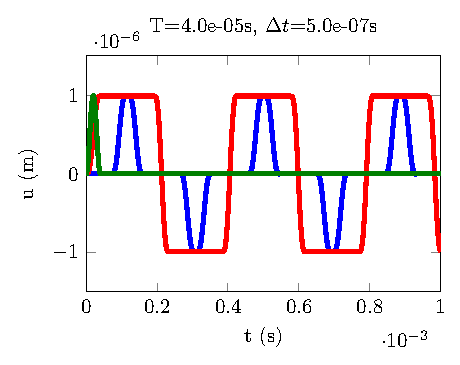
\includegraphics[width=0.40\linewidth]{Images/Choc/CalculSchem3.T1.dt5e-07.tikz.eps}}
\caption{Influence of $\Delta t$ on numerical integration, 
\\ Newmark scheme - Average acceleration 
\\ Fixed $T$ variable $\Delta t$
\label{InfluenceTimestepOnIntegration}}
\end{figure}

In order to avoid or reduce the presence of such perturbation we can change the integration scheme. The curves in the Figure \ref{DifferentIntegrationSchemes} represent the same as previously, but this time the loading and the time step stay the same and only the integration scheme changes. On the first graph then Newmark method : average acceleration is used. On the second it still is Newmark but it is called average acceleration modified, which can introduce dumping when the previous one is conservative. It does avoid to introduce high frequency perturbation but it changes the global solution by introducing a dumping effect regardless of the dumping defined for the mechanical system. The third graph is obtained with the HHT scheme, it allows to reduce the dumping effect to high frequency. Unfortunately the frequencies affected are linked to the time step which can be set by other parameters, moreover the result is a compromise between the two previous solutions, and it has just faded the perturbation slightly. Finally on the fourth part is the result given by the time discontinuous Galerkin method. It seems to be the less perturbed solution and the closest to what was obtained by increasing the time representation precision.
\begin{figure}[!ht]
\centering
\subfigure{\includegraphics[width=0.40\linewidth]{Images/Choc/CalculSchem3b.T1.tikz.eps}}
\hspace{0.5cm}
\subfigure{\includegraphics[width=0.40\linewidth]{Images/Choc/CalculSchem4.T1.tikz.eps}}
\subfigure{\includegraphics[width=0.40\linewidth]{Images/Choc/CalculSchem5.T1.tikz.eps}}
\hspace{0.5cm}
\subfigure{\includegraphics[width=0.40\linewidth]{Images/Choc/CalculSchem6.T1.tikz.eps}}
\caption{Use of different integration schemes
\\ Fixed $T$=4e-5s fixed $\Delta t$ =4e-6
\label{DifferentIntegrationSchemes}}
\end{figure}
\FloatBarrier


\subsection{PGD} 


\subsubsection{Problem definition}

\begin{itemize*}
\item Kinematic admissibility:
	$U \in [H^1(\Omega)]^3, U_{|\partial \Omega_U} = U_d $
\item Static admissibility:
	$ div \sigma + f_v = \rho \ddot{U} + \mu \dot{U}$ on $\Omega$ 
		and $\sigma . n _{|\partial \Omega_f} = f_d$
\item Behavior relation:
	$\sigma = H: \varepsilon (U)$ on $ \Omega$
\item Initial conditions:
	$U(0) = U_0$ and $ \dot{U}(0) = \dot{U}_0$
\end{itemize*}

Variational formulation: 
\begin{equation}
	\begin{array}{r l}
	\displaystyle
	\forall U^* ~ \text{KA to 0,} &
	\displaystyle
		\int_\Omega [\varepsilon (U^*): \sigma   
					+ U^* \mu \dot{U} 
					+ U^* \rho \ddot{U}
					- U^* f_d
					] d \Omega	
		\\ &
	\displaystyle
	- \int_{\partial \Omega_f} U^* f_d  ds		
		- \underbrace{
			\int_{\partial \Omega_U} U^* \sigma . n ds	
		  }_{=0}
		= 0
		\end{array}
		\label{VarationalFormulation}
\end{equation}

Where
\begin{itemize*}
\item $U$ is displacement
\item $\Omega$ space, with the boundary $\partial \Omega = \partial \Omega_U \cap \partial \Omega_f$
\item $\sigma$ stress tensor
\item $\varepsilon$ strain tensor
\item $\rho$ volumetric mass density
\item $\mu$ volumetric dumping (it is generally badly known)
\item $H$ Hook tensor
\item $f_v$ volumetric force
\item $f_d$ load on $\partial \Omega_f$
\end{itemize*}

%\begin{itemize*}
%\item $U$ est le déplacement
%\item $\Omega$ l'espace, avec le bord $\partial \Omega = \partial \Omega_U \cap \partial \Omega_f$
%\item $\sigma$ le tenseur des contraintes
%\item $\varepsilon$ le tenseur des déformations
%\item $\rho$ la masse volumique
%\item $\mu$ l'amortissement volumique (cette donnée est généralement mal connue)
%\item $H$ le tenseur de Hook
%\item $f_v$ effort volumique
%\item $f_d$ effort imposé sur $\partial \Omega_f$
%\end{itemize*}
%\vspace{0.3cm}

We use the PGD representation with separated variables:
\begin{equation}
	U(x,t,\theta) = \sum_{k=1}^n \varphi_k(x) g_k(t)h_k(\theta)
\end{equation}

Introducing this form in the problem defined in the equation \ref{VarationalFormulation}, we can obtain the three separated problems that will be solved each at a time for every iteration of the fixed point. These problems are described above.

%Where
%\begin{itemize*}
%\item $x$ is the space variable
%\item $t$ is the time variable
%\item $\theta$ a variable in parameter used here as an example
%\end{itemize*}

Let's discretize space to introduce the usual notations.
\begin{equation}
	\begin{array}{l c l c l}
		\varphi(x) &=& \sum_{i=1}^{Nbc_x}  N_i (x) \varphi_i &=& N_\varphi(x) \boldsymbol{\varphi_q} \\
	\end{array}
\end{equation}

%Where $Nbc_x$ représente le nombre de composante de discrétisation spatiale, l'indice $q$ représente le vecteur sur le domaine discrétisé.

In the variational formulation is replaced, $U^* $ by $ (\varphi gh)^* = ( \varphi^*gh+\varphi g^*h+\varphi gh^*) $.

And to simplify equation the usual notations for quantities integrated on the space domain are defined, $\mathbf{K}$ for the stiffness, $\mathbf{C}$ for dumping, $\mathbf{M}$ for the mass and $\mathbf{f}$ for the effort.
%\begin{equation}
%\mathbf{K} = \int_\Omega \varepsilon (N_\varphi(x)): H: \varepsilon (N_\varphi(x))~~dx
%\end{equation}
%\begin{equation}
%\mathbf{C} = \int_\Omega N_\varphi(x) \mu  N_\varphi(x)~~dx
%\end{equation}
%\begin{equation}
%\mathbf{M} = \int_\Omega N_\varphi(x) \rho  N_\varphi(x)~~dx
%\end{equation}
%\begin{equation}
%\mathbf{f} = \int_\Omega N_\varphi(x) f_v ~~dx 
%	%+ \int_{\partial \Omega_U} U_d (H: \varepsilon (N_\varphi(x)) . n) 
%	+ \int_{\partial \Omega_f} N_\varphi(x) f_d ~ds dt d\theta
%\end{equation}

And the result with all calculations done is : $\forall\boldsymbol{\varphi_q}^*$, $\forall g^*$, $\forall h^*$
\begin{equation}
\begin{array}{l}
	\displaystyle	
	\int_T \! \int_\Theta	\!\!
		\big(\boldsymbol{\varphi_q}^*gh + \boldsymbol{\varphi_q}g^*h + \boldsymbol{\varphi_q}gh^*\big)^T \!
					\bigg[~\mathbf{K}~ \boldsymbol{\varphi_q}gh
						+ ~\mathbf{C}~ \boldsymbol{\varphi_q} \dot{g}h 
						+ ~\mathbf{M}~ \boldsymbol{\varphi_q} \ddot{g}h
	\\ 
	  \displaystyle
		\phantom{\int_T\int_\Theta\big(\boldsymbol{\varphi_q}^{*T}gh + \boldsymbol{\varphi_q}g^*h + \boldsymbol{\varphi_q}gh^*}
			+ \mathbf{K} \sum_{k=1}^{n-1} (\boldsymbol{\varphi_q})_k       g_k  h_k 
			+ \mathbf{C} \sum_{k=1}^{n-1} (\boldsymbol{\varphi_q})_k  \dot{g_k} h_k 
	\\ \displaystyle
	  
		\phantom{\int_T\int_\Theta\big(\boldsymbol{\varphi_q}^{*T}gh + \boldsymbol{\varphi_q}g^*h + \boldsymbol{\varphi_q}gh^*} 
			+ \mathbf{M} \sum_{k=1}^{n-1} (\boldsymbol{\varphi_q})_k \ddot{g_k} h_k
			-\mathbf{f}~\bigg] ~dt d\theta
	= 0
\end{array}
\end{equation}
From which a problem is extracted for each variable.

\subsubsection{Space problem}

\begin{equation}
\begin{array}{r r l}
	& \displaystyle
		\int_T \! \int_\Theta
			gh [& \mathbf{K}~ gh
				+ ~\mathbf{C}~ \dot{g}h 
				+ ~\mathbf{M}~ \ddot{g}h
				] ~dt d\theta 
	~ \boldsymbol{\varphi_q}
	\\
	= &- \displaystyle
		\int_T \! \int_\Theta		
			gh [&  \mathbf{K} \sum_{k=1}^{n-1} (\boldsymbol{\varphi_q})_k       g_k  h_k 
				+ ~\mathbf{C} \sum_{k=1}^{n-1} (\boldsymbol{\varphi_q})_k  \dot{g_k} h_k 
		\\ &&
				+ ~\mathbf{M} \sum_{k=1}^{n-1} (\boldsymbol{\varphi_q})_k \ddot{g_k} h_k
				- ~\mathbf{f}] ~dt d\theta				
\end{array}
\end{equation}
So here is basically a problem in the form of linear system : $\boldsymbol{A}\times \boldsymbol{x}=\boldsymbol{b}$
%System to which boundary conditions need to be added by any method, as substitution or Lagrange multipliers. In the second case it would
%
%\begin{equation}
%~\mathbf{M}=
%	\begin{bmatrix}
%	   \mathbf{M} & 0 \\
%	   0 & 0 \\
%	\end{bmatrix}
%	\textrm{,  }
%	\mathbf{C}=
%	\begin{bmatrix}
%	   \mathbf{C} & 0 \\
%	   0 & 0 \\
%	\end{bmatrix}
%	\textrm{,  } 
%	\mathbf{K}=
%	\begin{bmatrix}
%	   \mathbf{K} & \mathbf{D}^T \\
%	   \mathbf{D} & 0 \\
%	\end{bmatrix}
%	\textrm{,  }
%	\boldsymbol{\varphi_q}=
%	\begin{bmatrix}
%	   \boldsymbol{\varphi_q} \\
%	   \boldsymbol{\lambda}\\
%	\end{bmatrix}
%	\textrm{ et }
%	\mathbf{f}=
%	\begin{bmatrix}
%	   \mathbf{f} \\
%	   \mathbf{b} \\
%	\end{bmatrix}
%\end{equation}
%Où $\mathbf{D}$ et $\mathbf{b}$ représentent les déplacement imposés de la manière suivante:
%$\mathbf{D} \boldsymbol{\varphi_q}= \mathbf{b}$.

\subsubsection{Time problem}

\begin{equation}
\begin{array}{r r l}
	&& \displaystyle
		\int_\Theta		
			\boldsymbol{\varphi_q}^Th [    ~\mathbf{K}~ \boldsymbol{\varphi_q}h ] ~d\theta
	~g
	+ 
		\int_\Theta		
			\boldsymbol{\varphi_q}^Th [ ~\mathbf{C}~ \boldsymbol{\varphi_q}h ] ~d\theta
	  ~\dot{g}
	\\ && \displaystyle	
	+ 
		\int_\Theta		
			\boldsymbol{\varphi_q}^Th [ ~\mathbf{M}~ \boldsymbol{\varphi_q}h ] ~d\theta
	  ~\ddot{g}
	\\
	= &-& \displaystyle
		\int_\Theta		
			\boldsymbol{\varphi_q}^Th [  \mathbf{K}~ \sum_{k=1}^{n-1} (\boldsymbol{\varphi_q})_k       g_k  h_k 
				+ ~\mathbf{C}~ \sum_{k=1}^{n-1} (\boldsymbol{\varphi_q})_k  \dot{g_k} h_k 

	\\ && \displaystyle
			\phantom{\int_\Theta		
			\boldsymbol{\varphi_q}^Th [  }
				+ ~\mathbf{M}~ \sum_{k=1}^{n-1} (\boldsymbol{\varphi_q})_k \ddot{g_k} h_k
				- ~\mathbf{f}~ ] ~d\theta
\end{array}
\end{equation}

What we find here is a differential equation in $g$, that can be solved like a classical dynamics problem, i.e. using an integration scheme like the ones discussed in the preceding section. 
%On se trouve donc en présence d'une équation différentielle en $g$, que l'on peut résoudre comme on résout classiquement un problème de dynamique, i.e. en utilisant un schéma d'intégration comme il en est question dans la section précédente. On peut aussi choisir résoudre en utilisant des élément finis temporels, le calcul est fournis en annexes.

\subsubsection{Parameter problem}

\begin{equation}
\begin{array}{r r l}
	&& \displaystyle
		\int_T
			\boldsymbol{\varphi_q}^Tg [  ~\mathbf{K}~ \boldsymbol{\varphi_q} g
				+ ~\mathbf{C}~ \boldsymbol{\varphi_q} \dot{g}
				+ ~\mathbf{M}~ \boldsymbol{\varphi_q} \ddot{g}
				] ~dt
	~ h
	\\
	= &-& \displaystyle
		\int_T
			\boldsymbol{\varphi_q}^Tg [  \mathbf{K}~ \sum_{k=1}^{n-1} (\boldsymbol{\varphi_q})_k       g_k  h_k 
				+ ~\mathbf{C}~ \sum_{k=1}^{n-1} (\boldsymbol{\varphi_q})_k  \dot{g_k} h_k 

		\\ &&
		\phantom{\int_T \boldsymbol{\varphi_q}^Tg [ }
				+ ~\mathbf{M}~ \sum_{k=1}^{n-1} (\boldsymbol{\varphi_q})_k \ddot{g_k} h_k
				- ~\mathbf{f}~] ~dt
\end{array}
\end{equation}
And finally, in this simple example where $\mathbf{K}$, $\mathbf{C}$ and $\mathbf{M}$ do not depend on the parameter, we find a scalar equation.

\subsection{Application onto academical problems}

\subsubsection{POD}
As said previously, the POD relies on a preceding resolution of a problem on the complete basis. The time sample on which the problem on complete basis is ran, is called snapshot. The reduce order modeling brought by the POD method allows to evaluate the system's response either on numerous similar problems or on the same problem as the snapshot but on a longer time. The snapshot, involving the model before reduction, can represent a heavy calculation, which would push toward a snapshot as short as possible. But its length is also linked to the quality of the modes found by the POD, which limits the will to shorten it. Here it was chosen long enough to capture several oscillations of the first mode. Beside its cost, the preceding resolution represents another drawback. Because it links the POD modes to a problem, and we have observed that changing parameters of the problem may reduce significantly the quality of the solution found. The POD being used here to give a comparison element for the PGD, its results will not be further developed.

\subsubsection{PGD}
%\label{ResultatsPGD}
%The PGD provides modes in space and time without preceding resolution on the complete basis, provides a solution, allows to add parameters, but it has a few weaknesses, particularly about convergence.
%
%Firstly, inside the fixed point loop, it can be noted that the fixed point does not converge every time quickly. And if the calculation is stopped after a fixed number of iterations ($k_{max}$ in  the algorithm \ref{AlgoPGD} in the section \ref{AlgoPGDPartie}), it can introduce a flawed mode, which can deteriorate the global solution and even prevent convergence. Fortunately it seems that normalizing space functions reduces the risks of it happening. The shape of the space mode is kept but not its intensity, which is reverberated on the time function.
%
%The Figure \ref{ConvergenceDuPointFixe} is based on a PGD resolution of a problem. The solution is constructed as a sum of products of functions of time and functions of space. The curve is an indication of the convergence of a fixed point. It is obtained with the following formula calculated at each iteration.
%
%\begin{equation}
%\left[
%\frac{\displaystyle 
%	\int_T \big(g_k(t) - g_{k-1}(t)\big)^2 dt  
%		~~\big((\boldsymbol{\varphi_q})_k - (\boldsymbol{\varphi_q})_{k-1}\big)^T 
%						\mathbf{K} 
%		  \big((\boldsymbol{\varphi_q})_k - (\boldsymbol{\varphi_q})_{k-1}\big)
%}
%{\displaystyle 
%\int_T g_k(t)^2 dt
%	~~(\boldsymbol{\varphi_q})_k^T \mathbf{K} (\boldsymbol{\varphi_q})_k
%} 
%\right]^\frac{1}{2}
%\end{equation}
%
%Which corresponds to:
%
%\begin{equation}
%\frac{\displaystyle 
%	\big\Vert (g_k - g_{k-1})\big\Vert_T 
%		~~\big\Vert (\boldsymbol{\varphi_q})_k 
%					- (\boldsymbol{\varphi_q})_{k-1} \big\Vert_\Omega
%}
%{\displaystyle 
%	\big\Vert g_k \big\Vert_T 
%		~~\big\Vert (\boldsymbol{\varphi_q})_k \big\Vert_\Omega 
%} 
%\end{equation}
%
%
%\begin{figure}[!ht]
%\centering
%\includegraphics[width=0.425\linewidth]{Images/PointFixe.tikz.eps}
%\caption{Fixed point convergence for a reluctant mode \label{ConvergenceDuPointFixe}}
%\end{figure}
%
%On the Figure \ref{ConvergenceDuPointFixe} we can notice that even after $8$ iterations of the fixed point, the mode can still present great variations. This mode has been chosen to illustrate the problem but most of them have converged after a few iterations. In the case where the fixed point did not converge, that may lead to a mode representing badly the system, we expect the next modes to bring a correction. It seems to be working provided that the space modes are normed.

The Figure \ref{NumberOfPGDModesNecessary} graphs are plotting the error of the solution found by the PGD to dynamics problems described Figure \ref{InfluenceLoadingVelocityOnIntegration}. What can be noticed is that the error level decreases slower as the loading is getting more "violent". Indeed the more violent the loading is, the closer it gets to a choc problem. Where the solution being a wave going through the material, it is not well represented by separated variables such as the PGD representation uses. It is showing a weakness of the PGD using a fixed point method to calculate new modes (which present an uncertainty of convergence), since we can see on the fourth graph that the method diverges. To avoid this possible problem the PGD can use another method called minimization \cite{nouy2010priori} that is assured to converge but is more costly in calculation.

\begin{figure}[!ht]
\centering
\subfigure{\includegraphics[width=0.40\linewidth]{Images/Choc/Error.CalculSchem3.T4.tikz.eps}}
\hspace{0.5cm}
\subfigure{\includegraphics[width=0.40\linewidth]{Images/Choc/Error.CalculSchem3.T3.tikz.eps}}
\subfigure{\includegraphics[width=0.40\linewidth]{Images/Choc/Error.CalculSchem3.T2.tikz.eps}}
\hspace{0.5cm}
\subfigure{\includegraphics[width=0.385\linewidth]{Images/Choc/Error.CalculSchem3.T1.tikz.eps}}
\caption{Influence of loading velocity on PGD congergence\label{NumberOfPGDModesNecessary}}
\end{figure}

\subsubsection{Comparisons}

On the Figure \ref{ErrorEvolution} is displayed the evolution of an error indicator : the maximum of the local difference between the resolution and a reference solution, which can be written : $e_ {Max} = \left|\frac{ max(s_ {Ref} - s_ {Cal}) } {max(s_ {Ref}) - min(s_ {Ref})} \right| $. The reference solution here is the solution obtained classically, without a model order reduction method.

\begin{figure}[!ht]
\centering
\subfigure{\includegraphics[width=0.45\linewidth]{Images/Calcul100M.PGD.tikz.eps}}
\hspace{0.5cm}
\subfigure{\includegraphics[width=0.45\linewidth]{Images/Calcul100M.POD.tikz.eps}}
\caption{Evolution of an error indicator while increasing the number of modes\label{ErrorEvolution}}
\end{figure}

It can be noticed on the left graph of Figure \ref{ErrorEvolution}, that not every PGD mode brings the same contribution to the solution. When the right hand side graph shows for the POD an error decreasing 	continuously and quickly, the PGD encounters stages. The aspect of the POD graph reminds the optimality of the basis it gives, and the speed at which the error decreases is linked to the way singular values decrease. Now this graph is not discarding PGD against POD, it should be kept in mind that adding a mode to the PGD is just run another fixed point, when each point of the POD graph here has needed a separate resolution. The presence of stages on the PGD graph suggests that several modes produced by the method do not contribute much to the solution, probably because those modes must be highly correlated with preceding ones. And eventually, every once in a while a new mode is found that is not correlated to the preceding ones, and the error decreases drastically.

To see how the modes are correlated to each other, we can visualize the Modal Assurance Criterion (MAC \cite{allemang2003modal}) analysis of a family of modes. In the case of the POD it would be useless since as the name of the method says the modes given are orthogonal to each other. On the contrary, visualizing the MAC analysis of the PGD modes reveals how much they are correlated and reinforce the idea of a stagnation of the method by finding new modes that could be expressed by a combination of the previous ones. What is shown on Figure \ref{AnalyseDeMAC} is actually the MAC analysis allowing to visualize the correlation between the modes obtained by PGD and those obtained by POD. What we see is that on the hundred modes found here by the PGD, they only correspond to the first dozen of the ones found by the POD (Reminder : when the MAC value is $1$ the correlation is total, i.e. the modes are identical.).
In numerous cases in the use of the PGD method, the modes can be orthogonalized, which would prevent those correlations. But unfortunately, the use of more than two variables in the resolution (like the addition of parameters), makes orthogonalization difficult or practically impossible, so it will not be implemented here.

\begin{figure}[!ht]
\centering
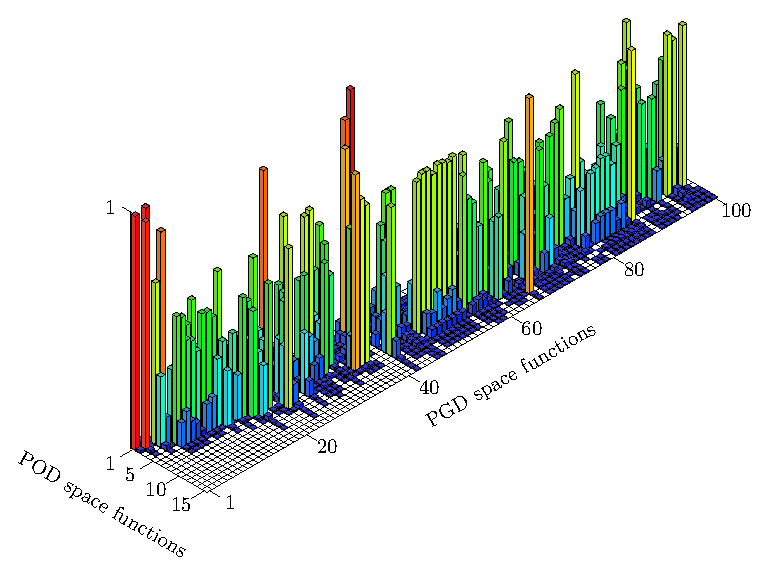
\includegraphics[width=0.8\linewidth]{Images/MAC.POD.PGD.eps}
\caption{Correlation between POD and PGD modes \label{AnalyseDeMAC}}
\end{figure}

\section{Conclusion}
The results presented showed that the PGD without the use of orthogonalization can present stagnation periods in the evolution of the solution, due to the creation of highly correlated modes. It was also highlighted that PGD presents a weakness, the more violent the loading gets the more modes are needed to reach a fixed quality for the solution. Moreover when high frequencies are appearing in transient dynamics the PGD can diverge, due to an inappropriate representation of waves with separated variables. And if we want to avoid to introduce perturbation that could cause convergence issues, the choice of an appropriate integration scheme must be done, depending on the problem treated. It seems that time discontinuous Galerkin is the one supporting the most abrupt cases. But as the industrial problem from which the project originated is in slow dynamics, it is not for sure the most relevant scheme to be used here. The other way to prevent divergence is to use the minimization method which will be used in the project in the future.
%(PGD is present in vibration calculation with the TVRC \cite{barbarulo2014proper})

\subsection{Prospect}
This work is part of a PhD, which takes place inside the MECASIF project, and its goal is to add the possibility to solve cases presenting localized non-linearities using the PGD. It is a real challenge because of the peculiar way the PGD finds a solution, and because the non-linearities will induce intrusive changes in the current program. The introduction of parameters is also planned in the near future, to treat the industrial case described in the introduction. 

%\begin{thebibliography}{99}
%
%\topsep=0.0ex
%\parsep=0.0ex
%\parskip=0.0ex
%\itemsep=0.0ex
%
%\bibitem{ref1} A.B. Normal,
%``My work with Dr Frankenstein'',
%Journal of Neurology, 6, 20-24, 1971.
%
%\end{thebibliography}

\section*{Acknowledgment}
This work was carried out as part of Project FUI AAP15 MECASIF  supported by the French "Fond Unique Interministériel".

\addcontentsline{toc}{part}{Bibliography} 
%\bibliographystyle{ieeetr}
\bibliographystyle{newsaxe}
\bibliography{References}

\end{document}



